\section{Analyse mathématique du système FHN}


%Diapo 1
\begin{frame}
\frametitle{Analyse mathématique du système FHN}
\framesubtitle{Système de FitzHugh-Nagumo : écriture et isoclines}
\begin{columns}
\column{0.5\textwidth}
\alert{\textbf{Le modèle à deux variables}}
\[
\begin{cases}
  \displaystyle \frac{dv}{dt} = v - \frac{v^3}{3} - w + I_{\text{app}} \\[8pt]
  \displaystyle \frac{dw}{dt} = \varepsilon (v + a - b w)
\end{cases}
\]
\alert{\textbf{Isoclines (nullclines)}}
\begin{itemize}
  \item $\dfrac{dv}{dt}=0 \; \implies ; w = v - \dfrac{v^3}{3} + I_{\text{app}}$ \hfill (cubique)
  \item $\dfrac{dw}{dt}=0 \; \implies ; w = \dfrac{v+a}{b}$ \hfill (droite)
\end{itemize}

\column{0.5\textwidth}
\centering
\begin{figure}
  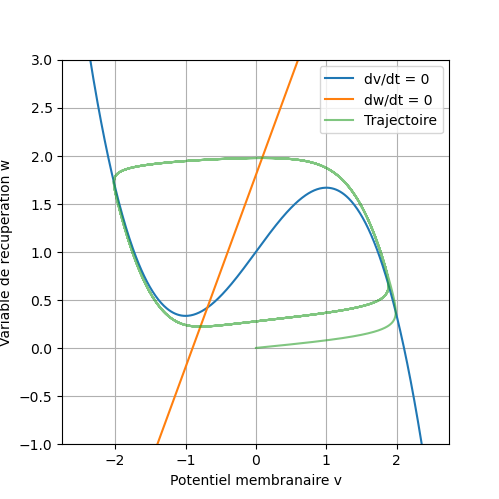
\includegraphics[width=\linewidth]{Figures/FHN.png}
  \caption{Portrait de phase du modèle de FitzHugh-Nagumo}
  %\source{ FitzHugh-Nagumo model, Scholarpedia, modifié d'après FitzHugh 1961}
\end{figure}
\end{columns}
\vspace{0.2cm}
\centerline{L’intersection des isoclines nulles donne le(s) point(s) fixe(s) du système.}
\end{frame}

%Diapo 2
\begin{frame}
\frametitle{Analyse mathématique du système FHN}
\framesubtitle{Point(s) fixe(s) et stabilité linéaire}
\begin{itemize}
  \item \alert{Point(s) fixe(s) :} intersection des deux isoclines nulles.
  \[
  \begin{cases}
    w^* = v^* - \dfrac{v^{*3}}{3} + I_{\text{app}} \\[6pt]
    w^* = \dfrac{v^*+a}{b}
  \end{cases}
  \]
  \item Suivant $I_{\text{app}}$ (ou $a$), on obtient 1 ou 3 points fixes.
  \item On se place ici dans le cas usuel d’un point fixe unique.
\end{itemize}

\alert{Linéarisation autour du point fixe $(v^*,w^*)$}
\[
\mathbf{J} = \begin{pmatrix}
  1 - v^{*2} & -1 \\
  \varepsilon & -\varepsilon b
\end{pmatrix}
\]
\begin{itemize}
  \item Trace : $\operatorname{tr}(\mathbf{J}) = 1 - v^{*2} - \varepsilon b$
  \item Déterminant : $\det(\mathbf{J}) = \varepsilon\bigl[1 + b(v^{*2}-1)\bigr]$
\end{itemize}
\end{frame}

%Diapo 3
\begin{frame}
\frametitle{Analyse mathématique du système FHN}
\framesubtitle{Stabilité et nature du point fixe}

\alert{\textbf{Conditions de stabilité (Routh-Hurwitz en 2D)}}
\begin{itemize}
  \item Un point fixe est \textbf{asymptotiquement stable} ssi 
  \(\operatorname{tr}(\mathbf{J}) < 0\) \textbf{et} \(\det(\mathbf{J}) > 0\).
  \item Ici, \(\det(\mathbf{J}) > 0\) pour les paramètres biologiques usuels (pas de point selle).
  \item La stabilité est donc gouvernée par le \textbf{signe de la trace}.
\end{itemize}

\alert{\textbf{Valeurs propres et classification}}
\[
\lambda_{\pm} = \frac{\operatorname{tr}(\mathbf{J}) \pm \sqrt{\Delta}}{2}, \quad
\Delta = \operatorname{tr}(\mathbf{J})^2 - 4\det(\mathbf{J})
\]
\begin{itemize}
  \item \(\operatorname{tr} < 0\) et \(\Delta > 0\) : \textbf{nœud stable} (amortissement monotone).
  \item \(\operatorname{tr} < 0\) et \(\Delta < 0\) : \textbf{foyer stable} (oscillations amorties).
  \item \(\operatorname{tr} > 0\) : \textbf{instable} (nœud ou foyer).  
  \item La frontière \(\operatorname{tr} = 0\) correspond à des valeurs propres imaginaires pures \(\Rightarrow\) \textbf{bifurcation de Hopf}.
\end{itemize}
\end{frame}


%Diapo 4
\begin{frame}
\frametitle{Analyse mathématique du système FHN}
\framesubtitle{Bifurcation de Hopf et naissance d’un cycle limite}
\alert{\textbf{Paramètre de bifurcation}} : $I_{\text{app}}$ ou $a$, ou $b$

Lorsque $I_{\text{app}}$ varie, le point fixe se déplace le long de la cubique.
\[
1 - v^{*2} = \varepsilon b \quad \text{(trace nulle)} \;\Longrightarrow\; \text{Bifurcation de Hopf.}
\]

\begin{itemize}
  \item Si $v^*$ est sur une \textbf{branche extérieure} ($|v^*|$ grand) : trace $<0$ $\rightarrow$ point fixe stable.
  \item Si $v^*$ est sur la \textbf{branche médiane} ($|v^*|$ petit, pente $>1$) : trace $>0$ $\rightarrow$ point fixe instable.
\end{itemize}

\alert{\textbf{Condition pour un cycle limite}}
\[
\varepsilon b < 1 \quad\text{(condition faible pour $\varepsilon$ petit)}
\]
Quand le point fixe devient instable, les trajectoires sont confinées par la cubique $\rightarrow$ un \textbf{cycle limite stable} apparaît (oscillations auto-entretenues).
\end{frame}